% Options for packages loaded elsewhere
\PassOptionsToPackage{unicode}{hyperref}
\PassOptionsToPackage{hyphens}{url}
\documentclass[
  ignorenonframetext,
  aspectratio=169,
]{beamer}
\newif\ifbibliography
\usepackage{pgfpages}
\setbeamertemplate{caption}[numbered]
\setbeamertemplate{caption label separator}{: }
\setbeamercolor{caption name}{fg=normal text.fg}
\beamertemplatenavigationsymbolsempty
% remove section numbering
\setbeamertemplate{part page}{
  \centering
  \begin{beamercolorbox}[sep=16pt,center]{part title}
    \usebeamerfont{part title}\insertpart\par
  \end{beamercolorbox}
}
\setbeamertemplate{section page}{
  \centering
  \begin{beamercolorbox}[sep=12pt,center]{section title}
    \usebeamerfont{section title}\insertsection\par
  \end{beamercolorbox}
}
\setbeamertemplate{subsection page}{
  \centering
  \begin{beamercolorbox}[sep=8pt,center]{subsection title}
    \usebeamerfont{subsection title}\insertsubsection\par
  \end{beamercolorbox}
}
% Prevent slide breaks in the middle of a paragraph
\widowpenalties 1 10000
\raggedbottom
\AtBeginPart{
  \frame{\partpage}
}
\AtBeginSection{
  \ifbibliography
  \else
    \frame{\sectionpage}
  \fi
}
\AtBeginSubsection{
  \frame{\subsectionpage}
}
\usepackage{iftex}
\ifPDFTeX
  \usepackage[T1]{fontenc}
  \usepackage[utf8]{inputenc}
  \usepackage{textcomp} % provide euro and other symbols
\else % if luatex or xetex
  \usepackage{unicode-math} % this also loads fontspec
  \defaultfontfeatures{Scale=MatchLowercase}
  \defaultfontfeatures[\rmfamily]{Ligatures=TeX,Scale=1}
\fi
\usepackage{lmodern}
\ifPDFTeX\else
  % xetex/luatex font selection
\fi
% Use upquote if available, for straight quotes in verbatim environments
\IfFileExists{upquote.sty}{\usepackage{upquote}}{}
\IfFileExists{microtype.sty}{% use microtype if available
  \usepackage[]{microtype}
  \UseMicrotypeSet[protrusion]{basicmath} % disable protrusion for tt fonts
}{}
\makeatletter
\@ifundefined{KOMAClassName}{% if non-KOMA class
  \IfFileExists{parskip.sty}{%
    \usepackage{parskip}
  }{% else
    \setlength{\parindent}{0pt}
    \setlength{\parskip}{6pt plus 2pt minus 1pt}}
}{% if KOMA class
  \KOMAoptions{parskip=half}}
\makeatother
\usepackage{longtable,booktabs,array}
\usepackage{caption}
\captionsetup[table]{skip=6pt}
\newcounter{none} % for unnumbered tables
\usepackage{calc} % for calculating minipage widths
\usepackage{caption}
% Make caption package work with longtable
\makeatletter
\def\fnum@table{\tablename~\thetable}
\makeatother
\usepackage{graphicx}
\makeatletter
\newsavebox\pandoc@box
\newcommand*\pandocbounded[1]{% scales image to fit in text height/width
  \sbox\pandoc@box{#1}%
  \Gscale@div\@tempa{\textheight}{\dimexpr\ht\pandoc@box+\dp\pandoc@box\relax}%
  \Gscale@div\@tempb{\linewidth}{\wd\pandoc@box}%
  \ifdim\@tempb\p@<\@tempa\p@\let\@tempa\@tempb\fi% select the smaller of both
  \ifdim\@tempa\p@<\p@\scalebox{\@tempa}{\usebox\pandoc@box}%
  \else\usebox{\pandoc@box}%
  \fi%
}
% Set default figure placement to htbp
\def\fps@figure{htbp}
\makeatother
\setlength{\emergencystretch}{3em} % prevent overfull lines
\providecommand{\tightlist}{%
  \setlength{\itemsep}{0pt}\setlength{\parskip}{0pt}}
% Auto-generated by infrastructure/rendering/_pdf_latex_helpers.py::extract_math_font_preamble.
% Minimal header passed to Pandoc via -H so Beamer slides pick up the same math font
% as the combined-PDF path. Adjust the manuscript's preamble.md to change the font globally.
\usepackage{unicode-math}
\setmathfont{latinmodern-math.otf}

% Manuscript macro/package fallbacks (newcommand -> providecommand).
% Core mathematics
\usepackage{amsmath}
\usepackage{amssymb}
% Document layout
% Tables
\usepackage{booktabs}
% Caption styling (booktabs already loaded above). Small caption font with a
% bold label ("Figure 1", "Table 2") gives the math/figure-heavy layout a
% consistent, journal-like caption rhythm without fighting pandoc-crossref —
% pandoc emits standard \caption{}, and caption/captionsetup only restyle it.
% ── Theorem environments ─────────────────────────────────────────────────
% amsthm is loaded above. The FedGVI<->Friston bridge is stated as a small
% number of theorems/definitions/lemmas/propositions/corollaries; sharing one
% counter (definition/lemma/proposition/corollary all step the `theorem`
% counter) gives a single monotone numbering 1, 2, 3, ... across all kinds, so
% authors can reference them as Theorem 1, Definition 2, Corollary 3 without a
% per-kind counter drifting out of order. Plain style for theorem-like results,
% definition style (upright body) for definitions.
% (algorithm2e intentionally not loaded: this manuscript states results as
% numbered amsthm Theorems/Definitions, not algorithm2e pseudocode.)
% Code listings
\usepackage{listings}
% Typography and formatting
% (siunitx intentionally not loaded: no \SI/\num units appear in this manuscript.)
% Cross-references and citations
% (cleveref and titlesec intentionally not loaded: unavailable in this TeX tree
% and not required. Cross-references resolve through pandoc-crossref's own
% \ref-style names — no \cref appears — and section heading styling falls back
% to the pandoc/LaTeX defaults.)
% ── TeX Live Basic-compatible mono font for code listings ────────────
% Latin Modern Mono is bundled with TeX Live Basic and keeps the manuscript
% renderable on minimal TeX installations. Mathematical Unicode coverage is
% provided separately by Latin Modern Math below, so the code font does not
% need a private JuliaMono installation.
%
% Use the TeX font filename rather than the system-family name: the minimal
% TeX Live fontconfig database may not register the OpenType family even though
% kpsewhich can resolve the bundled files.
% Math font for unicode-math: Latin Modern Math (TeX Live) has full BMP
% coverage including U+2223 (\mid), U+226A/226B (\ll/\gg), and the Greek/
% blackboard letters used in equations. Without an explicit \setmathfont,
% unicode-math falls back to lmroman text font which lacks several glyphs
% and emits "Missing character" warnings on every \mid in math mode.

% Slide layout defaults for warning-clean scientific decks.
\usepackage{etoolbox}
\IfFileExists{xurl.sty}{\usepackage{xurl}}{}
\IfFileExists{seqsplit.sty}{\usepackage{seqsplit}}{\newcommand{\seqsplit}[1]{#1}}
\protected\def\breakseq#1{\seqsplit{#1}}
\protected\def\breaktt#1{\begingroup\ttfamily\seqsplit{#1}\endgroup}
\setlength{\emergencystretch}{6em}
\tolerance=5000
\hbadness=10000
\hfuzz=1pt
\setlength{\tabcolsep}{2pt}
\AtBeginEnvironment{longtable}{\tiny\renewcommand{\arraystretch}{0.86}\setlength{\tabcolsep}{1pt}}
\AtBeginEnvironment{tabular}{\tiny\renewcommand{\arraystretch}{0.86}\setlength{\tabcolsep}{1pt}}
\AtBeginEnvironment{equation}{\tiny}
\AtBeginEnvironment{equation*}{\tiny}
\AtBeginEnvironment{align}{\tiny}
\AtBeginEnvironment{align*}{\tiny}
\AtBeginEnvironment{itemize}{\footnotesize}
\AtBeginEnvironment{enumerate}{\footnotesize}
\AtBeginEnvironment{description}{\footnotesize}
\setbeamerfont{caption}{size=\tiny}
\setbeamerfont{caption name}{size=\tiny}
\setbeamerfont{normal text}{size=\small}
\setbeamerfont{frametitle}{size=\small}
\setbeamerfont{section title}{size=\footnotesize}
\setbeamerfont{subsection title}{size=\footnotesize}
\setbeamertemplate{section page}{%
  \centering
  \begin{beamercolorbox}[sep=12pt,center,wd=\paperwidth]{section title}
    \parbox{0.86\paperwidth}{\centering\usebeamerfont{section title}\insertsection\par}
  \end{beamercolorbox}
}
\setbeamertemplate{subsection page}{%
  \centering
  \begin{beamercolorbox}[sep=8pt,center,wd=\paperwidth]{subsection title}
    \parbox{0.86\paperwidth}{\centering\usebeamerfont{subsection title}\insertsubsection\par}
  \end{beamercolorbox}
}
\setlength{\abovecaptionskip}{2pt}
\setlength{\belowcaptionskip}{0pt}

% Natbib and cross-reference fallbacks — slides don't load natbib
% or cleveref, but combined-PDF manuscript prose may emit these
% commands. The fallback renders citations as a bracketed key list
% and cross-references as detokenized labels so slides don't fail on
% undefined control sequences or raw underscores. \providecommand is
% a no-op if packages load later.
\providecommand{\citep}[1]{[#1]}
\providecommand{\citet}[1]{#1}
\providecommand{\citealp}[1]{#1}
\providecommand{\citeauthor}[1]{#1}
\providecommand{\citeyear}[1]{#1}
\providecommand{\cref}[1]{\texttt{\detokenize{#1}}}
\providecommand{\Cref}[1]{\texttt{\detokenize{#1}}}
\providecommand{\crefrange}[2]{\texttt{\detokenize{#1}}--\texttt{\detokenize{#2}}}
\providecommand{\Crefrange}[2]{\texttt{\detokenize{#1}}--\texttt{\detokenize{#2}}}
\providecommand{\paragraph}[1]{\textbf{#1}\ }

% Opt-in accessible presentation profile.
\setbeamerfont{normal text}{size*={20pt}{24pt}}
\setbeamerfont{frametitle}{size*={28pt}{32pt}}
\setbeamerfont{section title}{size*={28pt}{32pt}}
\setbeamerfont{subsection title}{size*={28pt}{32pt}}
\setbeamerfont{caption}{size*={16pt}{19pt}}
\setbeamerfont{caption name}{size*={16pt}{19pt}}
\setbeamerfont{itemize/enumerate body}{size*={20pt}{24pt}}
\setbeamerfont{itemize/enumerate subbody}{size*={20pt}{24pt}}
\setbeamerfont{itemize/enumerate subsubbody}{size*={20pt}{24pt}}
\setbeamerfont{itemize item}{size*={20pt}{24pt}}
\setbeamerfont{itemize subitem}{size*={20pt}{24pt}}
\setbeamerfont{itemize subsubitem}{size*={20pt}{24pt}}
\setbeamerfont{description body}{size*={20pt}{24pt}}
\setbeamerfont{description item}{size*={20pt}{24pt}}
\setbeamerfont{quote}{size*={20pt}{24pt}}
\setbeamerfont{quotation}{size*={20pt}{24pt}}
\AtBeginEnvironment{longtable}{\fontsize{20pt}{24pt}\selectfont}
\AtBeginEnvironment{tabular}{\fontsize{20pt}{24pt}\selectfont}
\AtBeginEnvironment{equation}{\fontsize{20pt}{24pt}\selectfont}
\AtBeginEnvironment{equation*}{\fontsize{20pt}{24pt}\selectfont}
\AtBeginEnvironment{align}{\fontsize{20pt}{24pt}\selectfont}
\AtBeginEnvironment{align*}{\fontsize{20pt}{24pt}\selectfont}
\AtBeginEnvironment{itemize}{\fontsize{20pt}{24pt}\selectfont}
\AtBeginEnvironment{enumerate}{\fontsize{20pt}{24pt}\selectfont}
\AtBeginEnvironment{description}{\fontsize{20pt}{24pt}\selectfont}
\AtBeginDocument{\usebeamerfont{normal text}}
\newlength{\AFSlideTableWidth}
% The fixed footer reservation is calibrated with the semantic seven-line regular-body budget.
\setbeamertemplate{footline}{%
  \leavevmode\vbox{%
    \hbox{%
      \begin{beamercolorbox}[wd=\paperwidth,ht=16pt,dp=3pt,center]{author in head/foot}%
        \fontsize{16pt}{19pt}\selectfont Untagged PDF derivative \textbar\ \href{../web/index.html}{HTML reader}%
      \end{beamercolorbox}%
    }%
    \vskip6pt%
  }%
}
% Accessible footer reserved height: 25pt.

\newtheorem{proposition}{Proposition}
\newtheorem{hypothesis}{Hypothesis}
\newtheorem{remark}[theorem]{Remark}
\newtheorem{axiom}{Axiom}
\newtheorem{property}{Property}
\usepackage{bookmark}
\IfFileExists{xurl.sty}{\usepackage{xurl}}{} % add URL line breaks if available
\urlstyle{same}
% fallback for those not using the hyperref driver hyperxmp:
\makeatletter
\@ifundefined{xmpquote}{\newcommand{\xmpquote}[1]{#1}}{}
\makeatother
\hypersetup{
  hidelinks,
  pdfcreator={LaTeX via pandoc}}

\author{\texorpdfstring{}{}}
\date{}

\begin{document}

\section{Formalism: recovery limits, EFE, and tempered
aggregation}\label{sec:formalism}

\begin{frame}{Formalism: recovery limits, EFE, and tempered aggregation}
\ifcsname proposition\endcsname
\else
\newtheorem{proposition}{Proposition}
\fi

The primitives of sec.~5 are governed by a compact set
of machine-checkable identities.
\end{frame}

\begin{frame}{Formalism: recovery\ldots{} (part 2)}
Their counter is monotone across the methods and this section.
Definitions 1 and 2 cover the
posterior and cavity / PVI update (sec.~5.3).
\end{frame}

\begin{frame}{Formalism: recovery\ldots{} (part 3)}
Lemma 3 gives the Rényi KL limit
(sec.~5.6).
\end{frame}

\begin{frame}{Formalism: recovery\ldots{} (part 4)}
Proposition 4 gives the \(\beta\)-loss and
rcce NLL limits (sec.~5.7). Theorem
5 and Corollary
6 give belief-sharing and Bayes recovery
(sec.~5.8).
\end{frame}

\begin{frame}[fragile]{Formalism: recovery\ldots{} (part 5)}
Proposition 7 below gives the
expected-free-energy identity.

Each carries a tested residual. None grants a bounded-influence
guarantee to the server-side \texttt{robust\_aggregate} heuristic; that
boundary is stated in sec.~3.3.
\end{frame}

\begin{frame}[fragile]{Recovery limits as the proof surface}
\protect\phantomsection\label{sec:formalism-recovery}
The recovery limits separate client and server claims. The divergence
and loss limits recover the standard-Bayes client update; the
independently tested identity equates \texttt{robust\_aggregate} with
\texttt{log\_linear\_pool} when \texttt{robustness=0}, recovering the
project's standard server pool.
\end{frame}

\begin{frame}{Recovery limits as the\ldots{} (part 2)}
Under the explicit shared-support, posterior-log-potential, and
fixed-weight assumptions in sec.~5.8, that pool
is a categorical specialization of Eq. 7's message-combination term, not
recovery of the complete source protocol (Friston et al. 2024).
\end{frame}

\begin{frame}{Recovery limits as the\ldots{} (part 3)}
We collect the five residuals that pin those limited claims, each
emitted by the test-suite and reported in
sec.~7.1, never hardcoded.
\end{frame}

\begin{frame}{Recovery limits as the\ldots{} (part 4)}
Read each row of the table below as a triple: the robust primitive, the
trusting knob value at which it must collapse onto its standard-Bayes or
project-local counterpart, and the tested residual measuring whatever
gap survives at that value. The rows differ in what kind of check they
are.
\end{frame}

\begin{frame}{Recovery limits as the\ldots{} (part 5)}
The divergence and loss rows evaluate inside the implementation's
closed-form switch band, so their zeros are exact branch identities ---
guaranteed by construction, not measurements that could have come out
otherwise.
\end{frame}

\begin{frame}{Recovery limits as the\ldots{} (part 6)}
Their genuine falsifiers are the \emph{off-switch} convergence
residuals, evaluated just outside the band (at \(\alpha = 1.00001\),
\(\beta = 1.00 \times 10^{-6}\),
\(q_{\text{loss}} = 1.00 \times 10^{-6}\)) where the general formulas
run and a nonzero gap is possible: those residuals are
\(1.66 \times 10^{-5}\), \(1.24 \times 10^{-5}\),
\end{frame}

\begin{frame}{Recovery limits as the\ldots{} (part 7)}
and \(1.12 \times 10^{-5}\) respectively, and any failure of those
quantities to shrink toward the limit would falsify the containment
claim.
\end{frame}

\begin{frame}{Recovery limits as the\ldots{} (part 8)}
The posterior row is a measured identity on the general code path, so
its near-zero residual is itself the falsification surface. The
aggregate row's zero at exactly \(c=0\) is likewise branch-exact; the
identity is additionally exercised on the iterative code path at
near-zero robustness,
\end{frame}

\begin{frame}{Recovery limits as the\ldots{} (part 9)}
where the consensus must still land on the log-linear pool to tight
tolerance.
\end{frame}

\begin{frame}{Recovery limits as the\ldots{} (part 10)}
{\def\LTcaptype{none} % do not increment counter
% template-accessible-table-inset
\begingroup
\setlength{\AFSlideTableWidth}{\textwidth}%
\setlength{\LTleft}{\fill}%
\setlength{\LTright}{\fill}%
\begin{longtable}[]{@{}
  >{\raggedright\arraybackslash}p{(\AFSlideTableWidth - 4\tabcolsep) * \real{0.5510}}
  >{\raggedright\arraybackslash}p{(\AFSlideTableWidth - 4\tabcolsep) * \real{0.2449}}
  >{\raggedright\arraybackslash}p{(\AFSlideTableWidth - 4\tabcolsep) * \real{0.2041}}@{}}
\toprule\noalign{}
\begin{minipage}[b]{\linewidth}\raggedright
Identity (owner statement)
\end{minipage} & \begin{minipage}[b]{\linewidth}\raggedright
Trusting limit
\end{minipage} & \begin{minipage}[b]{\linewidth}\raggedright
Tested residual
\end{minipage} \\
\midrule\noalign{}
\endhead
Rényi \(\to\) KL (Lemma 3,
eq.~6) & \(\alpha \to 1\) & 0 \\
\bottomrule\noalign{}
\end{longtable}
\endgroup
}
\end{frame}

\begin{frame}[fragile]{Recovery limits as the\ldots{} (part 11)}
The central project identity is the aggregation collapse of
eq.~10: \texttt{robust\_aggregate(robustness=0)}
equals the log-linear pool eq.~9. Its source
bridge is deliberately narrow.
\end{frame}

\begin{frame}{Recovery limits as the\ldots{} (part 12)}
Take the admitted posteriors defined in
sec.~5.8, on a finite common support with
\(q_n(s)>0\), and represent each Eq. 7 softmax input as a posterior log
potential \(m_n(s)=\log q_n(s)+\kappa_n\), with \(\kappa_n\) constant in
\(s\) and fixed declared weights \(w_n\) independent of the emerging
consensus.
\end{frame}

\begin{frame}{Recovery limits as the\ldots{} (part 13)}
Softmax then cancels the additive constants and yields the project pool.
\end{frame}

\begin{frame}{Recovery limits as the\ldots{} (part 14)}
This identifies only the source equation's message-combination term; it
does not identify source message construction, cavity/exclusion policy,
scheduling, generative factors, or the complete protocol.
\end{frame}

\begin{frame}{Recovery limits as the\ldots{} (part 15)}
Theorem 5
(sec.~5.8) states that specialization and the
local \(c=0\) identity; the residual 0 above pins the latter.
\end{frame}

\begin{frame}[fragile]{Recovery limits as the\ldots{} (part 16)}
Corollary 6 establishes the separate client
result: \texttt{generalized\_posterior(KLD,\ NLL)} reproduces the
closed-form prior-times-likelihood Bayes posterior of
eq.~11 to residual 5.55e-17.
\end{frame}

\begin{frame}{Recovery limits as the\ldots{} (part 17)}
Pooling such local posteriors has the stated categorical specialization
only under the theorem's assumptions.
\end{frame}

\begin{frame}{Recovery limits as the\ldots{} (part 18)}
The honesty contract binds here: the theorem and corollary cover only
the recovery identity and the per-agent rigorous axis (Proposition
4); no statement transfers the
bounded-influence guarantee to the server-side divergence-reweighting
heuristic,
\end{frame}

\begin{frame}{Recovery limits as the\ldots{} (part 19)}
whose positive property is the \(\texttt{robustness}=0\) limit of
eq.~10. A scoped no-go rejects a declared
separable objective class without certifying another.
\end{frame}

\begin{frame}{Expected-free-energy identity as an algebraic check}
\protect\phantomsection\label{sec:formalism-efe}
The active-inference substrate that drives the studies of
sec.~7 is a categorical specialization of the
expected-free-energy algebra discussed by Friston et al. (Friston et al.
2024).
\end{frame}

\begin{frame}{Expected-free-energy\ldots{} (part 2)}
It decomposes the expected free energy of a policy \(\boldsymbol{\pi}\)
into two equivalent two-term forms.
\end{frame}

\begin{frame}{Expected-free-energy\ldots{} (part 3)}
The risk-plus-ambiguity (cost) view and the negated
pragmatic-plus-epistemic (value) view are the same scalar
\(G(\boldsymbol{\pi})\) rearranged (Da Costa et al. 2020; Friston et al.
2024):
\end{frame}

\begin{frame}{Expected-free-energy\ldots{} (part 4)}
\begin{equation}\tag{22}\protect\phantomsection\label{eq:efe-decomposition}{
\begin{aligned}
G(\boldsymbol{\pi})
&= \underbrace{\text{risk} + \text{ambiguity}}_{\text{cost view}}\\
&= -\underbrace{\big(\text{pragmatic} + \text{epistemic}\big)}_{\text{value view}}.
\end{aligned}
}\end{equation}
\end{frame}

\begin{frame}{Expected-free-energy\ldots{} (part 5)}
The two views are not approximations of one another; they are the same
scalar rearranged. In the implementation the shared entropy term enters
both sides of the rearrangement, so the identity residual is zero by
construction --- it is a definitional consistency check on the
decomposition's bookkeeping,
\end{frame}

\begin{frame}{Expected-free-energy\ldots{} (part 6)}
not an independent measurement.

The scientific content lives in the per-term semantics, which are pinned
independently of the identity (see the closing clause of the proposition
below):
\end{frame}

\begin{frame}{Expected-free-energy\ldots{} (part 7)}
\begin{equation}\tag{23}\protect\phantomsection\label{eq:efe-identity}{
\begin{aligned}
&\big(\text{risk} + \text{ambiguity}\big)\\
&\quad + \big(\text{pragmatic} + \text{epistemic}\big)
\equiv 0.
\end{aligned}
}\end{equation}
\end{frame}

\begin{frame}{Expected-free-energy\ldots{} (part 8)}
\begin{proposition}[Expected-free-energy decomposition identity]\label{prop:efe-decomposition}
For the categorical model in \texttt{expected\_free\_energy.py}, the cost and
negated-value forms of (22) give the same
$G(\boldsymbol{\pi})$; hence (23) holds to machine precision.
Cross-entropy and entropy splits establish the equality.
\end{proposition}
\end{frame}

\begin{frame}{Expected-free-energy\ldots{} (part 9)}
The residual is pinned to \(10^{-9}\). Independent checks require
deterministic likelihoods to give zero ambiguity, uninformative
likelihoods zero epistemic value, and preference-matched predictions
lower risk.
\end{frame}

\begin{frame}{Expected-free-energy\ldots{} (part 10)}
Here risk is \(\mathrm{KL}(q(o\mid\boldsymbol{\pi})\,\|\,p_C(o))\), and
ambiguity is expected likelihood entropy
\(\mathbb{E}_{q(s)}[H[p(o\mid s)]]\).
\end{frame}

\begin{frame}{Expected-free-energy\ldots{} (part 11)}
Pragmatic value is expected log-preference
\(\mathbb{E}_{q_{\boldsymbol{\pi}}(o)}[\ln p_C(o)]\). Epistemic value is
the state-outcome mutual information
\(H[q_{\boldsymbol{\pi}}(o)] - \mathbb{E}_{q(s)}[H[p(o\mid s)]]\).
\end{frame}

\begin{frame}{Expected-free-energy\ldots{} (part 12)}
The executed formal-specialization diagnostic of
fig.~8 uses a uniform prior over the nine locations.
This is intentional: the canonical sentinel-world \(D_0\) is a point
mass at the den,
\end{frame}

\begin{frame}{Expected-free-energy\ldots{} (part 13)}
and under that fully resolved prior the mutual-information term is zero
because there is no state uncertainty for an observation to reduce.
\end{frame}

\begin{frame}{Expected-free-energy\ldots{} (part 14)}
The uncertainty-bearing diagnostic makes the epistemic term visible
without changing the canonical \(D_0\) used by the inference and
recovery studies. Thus a near-zero epistemic value is a meaningful null
condition, not a missing term.
\end{frame}

\begin{frame}{Expected-free-energy\ldots{} (part 15)}
fig.~8 shows the additive risk-plus-ambiguity view
beside a signed pragmatic/epistemic waterfall whose terminal endpoint is
\(G(\boldsymbol{\pi})\), labels epistemic value as
\(I(s;o\mid\boldsymbol{\pi})\), and annotates the identity residual; it
visualizes Proposition 7,
\end{frame}

\begin{frame}{Expected-free-energy\ldots{} (part 16)}
not a fitted result, so it carries no error bars.
\end{frame}

\begin{frame}{Expected-free-energy\ldots{} (part 17)}
\begin{figure}
\centering
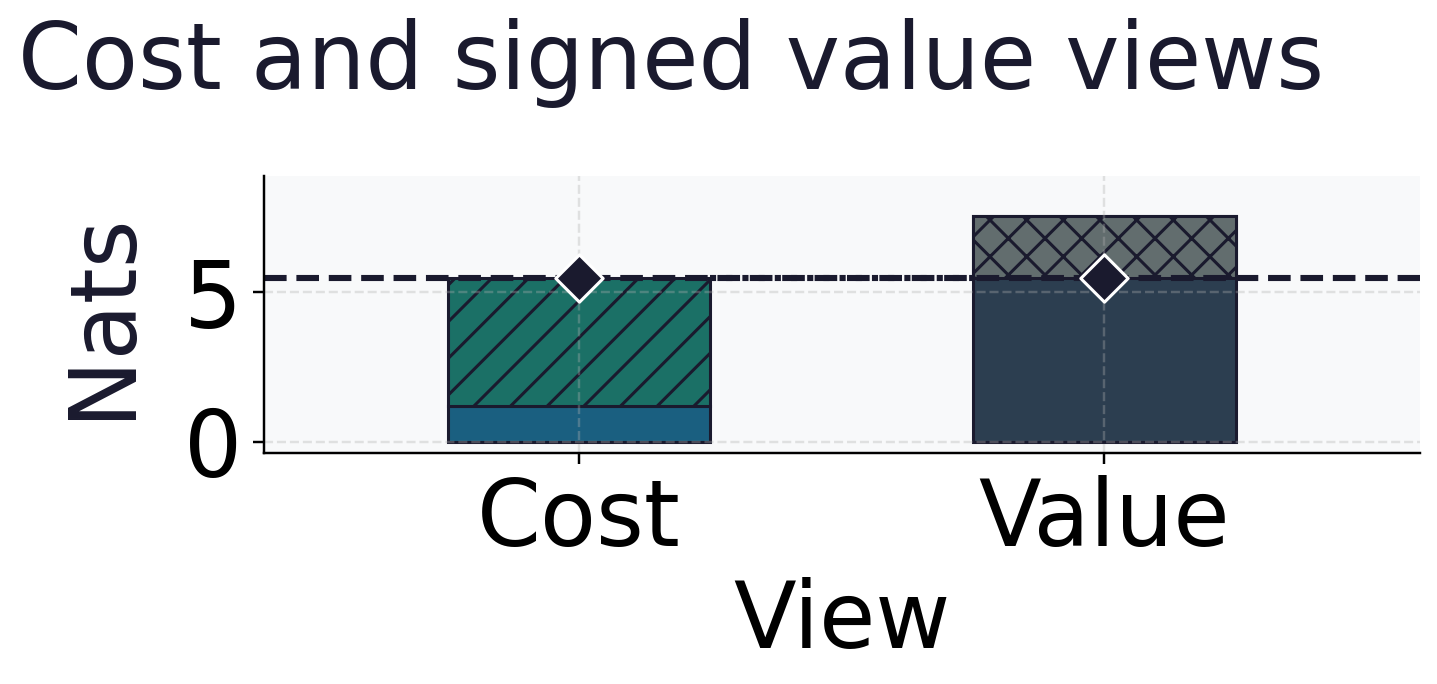
\includegraphics[keepaspectratio,width=0.98\linewidth,height=0.8\textheight,alt={Risk plus ambiguity and signed pragmatic minus epistemic waterfall share the same terminal G.}]{../figures/efe_decomposition.slide-identity.png}
\refstepcounter{figure}\label{fig:efe-decomp-slide-panel-1}
\end{figure}
\end{frame}

\begin{frame}{Expected-free-energy\ldots{} (part 18)}
\begin{figure}
\centering
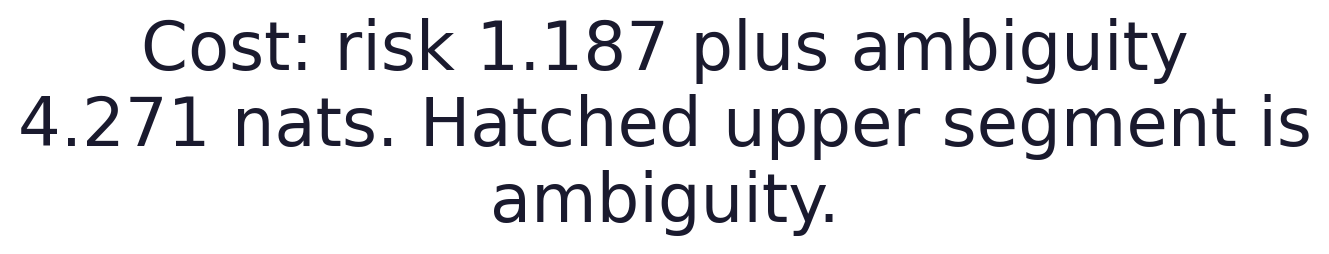
\includegraphics[keepaspectratio,width=0.98\linewidth,height=0.8\textheight,alt={Cost: risk 1.187 plus ambiguity 4.271 nats. Hatched upper segment is ambiguity.}]{../figures/efe_decomposition.slide-cost.png}
\refstepcounter{figure}\label{fig:efe-decomp-slide-panel-2}
\end{figure}
\end{frame}

\begin{frame}{Expected-free-energy\ldots{} (part 19)}
\begin{figure}
\centering
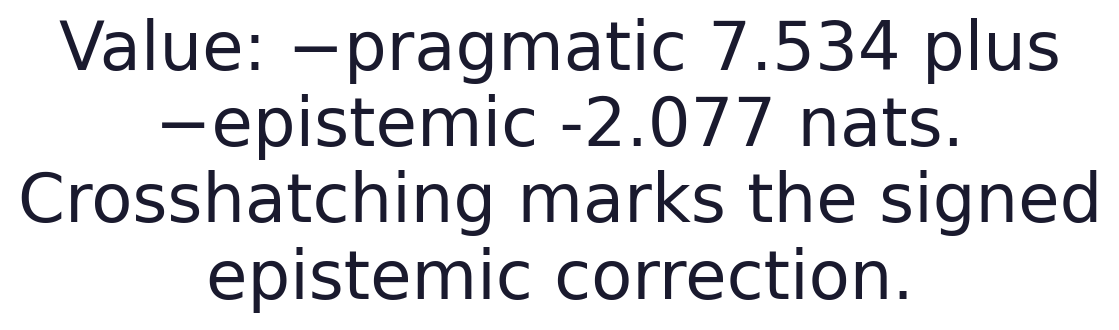
\includegraphics[keepaspectratio,width=0.98\linewidth,height=0.8\textheight,alt={Value: −pragmatic 7.534 plus −epistemic -2.077 nats. Crosshatching marks the signed epistemic correction.}]{../figures/efe_decomposition.slide-value.png}
\refstepcounter{figure}\label{fig:efe-decomp-slide-panel-3}
\end{figure}
\end{frame}

\begin{frame}{Expected-free-energy\ldots{} (part 20)}
\begin{figure}
\centering
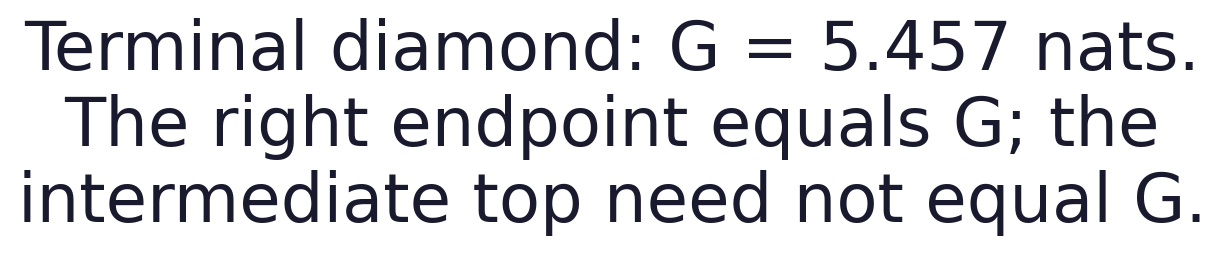
\includegraphics[keepaspectratio,width=0.98\linewidth,height=0.8\textheight,alt={Terminal diamond: G = 5.457 nats. The right endpoint equals G; the intermediate top need not equal G.}]{../figures/efe_decomposition.slide-endpoint.png}
\refstepcounter{figure}\label{fig:efe-decomp-slide-panel-4}
\end{figure}
\end{frame}

\begin{frame}{Expected-free-energy\ldots{} (part 21)}
\begin{figure}
\centering
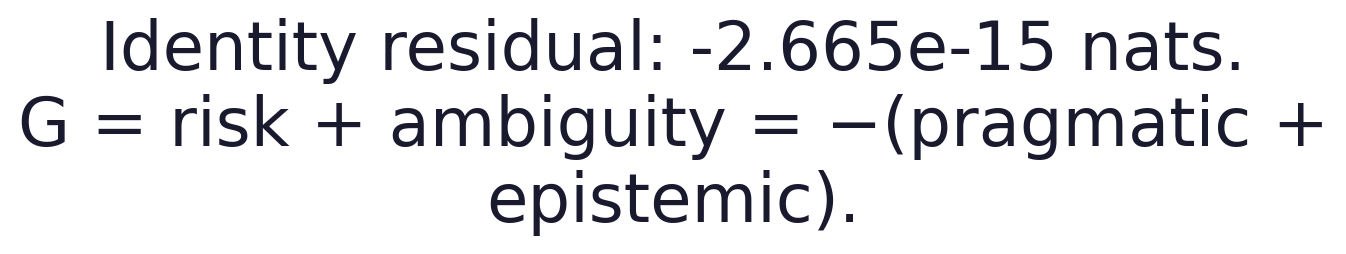
\includegraphics[keepaspectratio,width=0.98\linewidth,height=0.8\textheight,alt={Identity residual: -2.665e-15 nats. G = risk + ambiguity = −(pragmatic + epistemic).}]{../figures/efe_decomposition.slide-residual.png}
\refstepcounter{figure}\label{fig:efe-decomp-slide-panel-5}
\end{figure}
\end{frame}

\begin{frame}{Expected-free-energy\ldots{} (part 22)}
\begin{figure}
\centering

\includegraphics[keepaspectratio,width=0.98\linewidth,height=0.8\textheight,alt={Uniform diagnostic prior makes information gain visible. One categorical identity diagnostic; no stochastic replication or uncertainty interval.}]{../figures/efe_decomposition.slide-scope.png}
\refstepcounter{figure}\label{fig:efe-decomp-slide-panel-6}
\end{figure}
\end{frame}

\begin{frame}{Expected-free-energy\ldots{} (part 23)}
The expected-free-energy identity of eq.~23 is the
action-selection counterpart of the inference-side recovery limits
collected above: both are exact, closed-form, machine-checkable
identities over the same categorical generative model.
\end{frame}

\begin{frame}{Expected-free-energy\ldots{} (part 24)}
Together they establish that the FedGVI-federated active-inference
colony of this work is built on verified algebra throughout --- the
per-agent generalized-Bayes update recovers standard Bayes, the
aggregation recovers the project log-linear pool under its qualified
categorical bridge,
\end{frame}

\begin{frame}{Expected-free-energy\ldots{} (part 25)}
and the policy scoring decomposes exactly --- so every robustness result
in sec.~7 is a controlled departure from a known, tested
fixed point rather than an unmoored claim.
\end{frame}

\begin{frame}{Tempered aggregation free energy and the
accuracy-guarantee trade}
\protect\phantomsection\label{sec:formalism-tempered}
The recovery limits and the expected-free-energy identity fix the
\emph{endpoints} of the aggregation family; the remaining formal
question is what a controlled departure from the unit-entropy server
buys and what it costs.
\end{frame}

\begin{frame}{Tempered aggregation free\ldots{} (part 2)}
The objective-backed variational aggregator of
sec.~12 holds its consensus-entropy term at unit
weight.
\end{frame}

\begin{frame}{Tempered aggregation free\ldots{} (part 3)}
Freeing that single coefficient produces a one-parameter family whose
only moving part is the sharpness of the consensus, and whose raw
effective-weight bound is provably untouched. The following proposition
isolates exactly that separation --- algebra that moves versus algebra
that does not ---
\end{frame}

\begin{frame}{Tempered aggregation free\ldots{} (part 4)}
before the interpretation subsections turn to the empirical accuracy
question the algebra cannot settle on its own.
\end{frame}

\begin{frame}{Tempered aggregation free\ldots{} (part 5)}
\begin{proposition}[Tempered aggregation free energy]\label{prop:tempered-aggregation}
Let $\lambda > 0$ and let $F_\lambda$ be (30). At fixed $a$,
the $q$-minimizer is (31). At
$\lambda = 1.0$, $F_\lambda$ and both updates equal
the standard variational aggregate bit-for-bit. The $a$-update and bound
$a_n \le w_n$ omit $\lambda$ and hold for every $\lambda > 0$.
\end{proposition}
\end{frame}

\begin{frame}{Tempered aggregation free\ldots{} (part 6)}
At that default, the endpoint-selection rule also reduces bit-for-bit to
the standard variational aggregate (Definition
10; sec.~12).
\end{frame}

\begin{frame}{Tempered aggregation free\ldots{} (part 7)}
The proposition is intentionally more specific than the phrase
``temperature improves robustness.'' It identifies exactly which part of
the variational server changes when the entropy coefficient changes, and
it separates that algebra from the empirical accuracy question.
\end{frame}

\begin{frame}{Tempered aggregation free\ldots{} (part 8)}
The objective and its update rules are a generalized-Bayes construction
in the sense of (Bissiri et al. 2016; Knoblauch et al. 2022), while the
particular client/server decomposition is the one implemented and tested
here.
\end{frame}

\begin{frame}{What the entropy weight controls}
\protect\phantomsection\label{sec:formalism-tempered-interpretation}
For a fixed effective-weight vector \(a\) and \(\lambda>0\), the
\(q\)-block in eq.~31 is a weighted geometric
pool of the local posteriors with inverse temperature \(1/\lambda\).
Lower \(\lambda\) concentrates more sharply on states that receive
consistent log-belief support;
\end{frame}

\begin{frame}{What the entropy weight\ldots{} (part 2)}
larger \(\lambda\) spreads probability mass and retains more entropy.
\end{frame}

\begin{frame}{What the entropy weight\ldots{} (part 3)}
As \(\lambda\downarrow0\), the positive-temperature expression
approaches a winner-take-most consensus (subject to ties and finite
numerical support), whereas large \(\lambda\) approaches a flatter
distribution.
\end{frame}

\begin{frame}{What the entropy weight\ldots{} (part 4)}
The implementation exposes that endpoint as a separately defined
deterministic tied-argmax rule; it does not substitute \(\lambda=0\)
into the objective or coordinate update.

This is a controlled change in the consensus geometry, not an automatic
outlier detector.
\end{frame}

\begin{frame}{What the entropy weight\ldots{} (part 5)}
The coupling matters. Although the formula for the \(a\)-block does not
contain \(\lambda\), the fixed point can still change because \(a_n\) is
evaluated at the new \(q\).
\end{frame}

\begin{frame}{What the entropy weight\ldots{} (part 6)}
The correct statement is therefore conditional: for any current
consensus, the effective-weight update and the raw bound \(a_n\leq w_n\)
are unchanged; after alternating updates, different temperatures can
reach different coupled \((q,a)\) fixed points.
\end{frame}

\begin{frame}{What the entropy weight\ldots{} (part 7)}
This distinction prevents the temperature result from being read as a
theorem that the normalized influence or accuracy is invariant in
\(\lambda\).
\end{frame}

\begin{frame}{Recovery at the qualified log-linear-pool corner}
\protect\phantomsection\label{sec:formalism-tempered-recovery}
At the configured default \(\lambda=1.0\), the entropy coefficient is
the unit coefficient used by the original variational aggregator. The
implementation therefore recovers that aggregator bit-for-bit,
\end{frame}

\begin{frame}{Recovery at the qualified\ldots{} (part 2)}
including its block updates and its endpoint-selection rule.
\end{frame}

\begin{frame}{Recovery at the qualified\ldots{} (part 3)}
Turning the robustness strength \(c\) to zero then sets every server
weight to its base value and gives the tempered log-linear pool. At the
default temperature this is the ordinary log-linear pool of
eq.~9.
\end{frame}

\begin{frame}{Recovery at the qualified\ldots{} (part 4)}
Under the shared-support, posterior-log-potential, and fixed-weight
assumptions of sec.~5.8, that is the
categorical specialization of Eq. 7's message-combination term; it is
not the complete belief-sharing protocol of (Friston et al. 2024). Away
from that default,
\end{frame}

\begin{frame}{Recovery at the qualified\ldots{} (part 5)}
the result is a tempered generalization of the pool and should not be
described as Friston's Eq. 7 itself.
\end{frame}

\begin{frame}{Recovery at the qualified\ldots{} (part 6)}
This nested limit is useful for interpretation. The \(c\to0\) limit
identifies the aggregation family with a known consensus operator; the
\(\lambda=1.0\) slice identifies the objective-backed implementation
used in the main server comparison.
\end{frame}

\begin{frame}[fragile]{Recovery at the qualified\ldots{} (part 7)}
Neither limit grants the server-side \texttt{robust\_aggregate}
heuristic a variational objective or a bounded-influence guarantee. The
FedGVI literature's rate and robustness results remain attached to their
stated loss, divergence,
\end{frame}

\begin{frame}{Recovery at the qualified\ldots{} (part 8)}
and sampling assumptions (Mildner, Hamelijnck, et al. 2025; Mildner,
Giampouras, et al. 2025).
\end{frame}

\begin{frame}{What the accuracy--guarantee trade can establish}
\protect\phantomsection\label{sec:formalism-tempered-evidence}
The executed grid over \(\lambda\in\{0.1, 0.2, 0.3, 0.5, 0.7, 1\}\) is a
finite sensitivity study, not a search over a continuous optimum.
\end{frame}

\begin{frame}{What the\ldots{} (part 2)}
It asks whether any tested temperature narrows the point-accuracy gap to
the sharp heuristic while retaining the same effective-weight update.
The closest tested temperature is \(\lambda^{\ast}=0.3\),

with observed gap \(0.0008\).
\end{frame}

\begin{frame}{What the\ldots{} (part 3)}
These tokens are computed from the executed contaminated-colony trials
and are reported with the grid definition so a reader can reproduce the
selection rule.
\end{frame}

\begin{frame}{What the\ldots{} (part 4)}
The result has two distinct readings. If a lower temperature improves
the paired point-accuracy comparison, it provides design evidence that
entropy regularization can be tuned rather than accepted as a fixed
conservatism penalty.
\end{frame}

\begin{frame}{What the\ldots{} (part 5)}
If no tested temperature closes the gap, that negative result is still
informative: within this objective family, the same entropy mechanism
that keeps consensus diffuse can limit exact point recovery under
confident contamination.
\end{frame}

\begin{frame}{What the\ldots{} (part 6)}
In either case, the grid does not identify a universally best
temperature, establish minimax robustness, or transfer the variational
raw weight bound to a different estimator. Generalized-Bayes calibration
and robust-loss theory motivate the family,
\end{frame}

\begin{frame}{What the\ldots{} (part 7)}
but only the executed categorical design supports the present
finite-grid statement (Bissiri et al. 2016; Knoblauch et al. 2022;
Mildner, Hamelijnck, et al. 2025).
\end{frame}

\begin{frame}{Publication-facing interpretation}
\protect\phantomsection\label{sec:formalism-tempered-interpretation-summary}
The practical contract is consequently three-part. Use the default
temperature when exact compatibility with the tested variational server
is the priority.
\end{frame}

\begin{frame}{Publication-facing\ldots{} (part 2)}
Explore the declared grid when the application can trade concentration
against the same raw effective-weight control.
\end{frame}

\begin{frame}{Publication-facing\ldots{} (part 3)}
Treat any selected temperature as a configuration-specific empirical
choice until it is tested under a new contamination mechanism, colony
size, sensor model, or loss. This is the appropriate bridge between the
formal objective and the active-inference setting:
\end{frame}

\begin{frame}{Publication-facing\ldots{} (part 4)}
it exposes a tunable consensus geometry while keeping recovery,
guarantee, and accuracy claims on separate evidence tracks.
\end{frame}

\end{document}
